% LaTeX: figurer, tabeller, teoremer, matriser, pgfplots og opsjoner over flere linjer
\documentclass{article}
\usepackage{graphicx, booktabs, amsthm, pgfplots, xcolor, hyperref}
\hypersetup{
  colorlinks=true,
  linkcolor=rust, urlcolor=darkblue,
}
\pgfplotsset{baneplott/.style={grid=major, xmin=-12, xmax=4, axis equal image, xlabel={$x$ (\si{m})}}}
\definecolor{rust}{HTML}{99380E}
\newtheorem{teorem}{Teorem}
\newenvironment{oppgave}[1][]{\par\textbf{Oppgave #1}}{\par}
\begin{document}
\begin{figure}[htbp]
  \centering
  \includegraphics[width=0.8\linewidth, trim=0 10 0 0, clip]{figurer/bane.pdf}
  \caption{Banen til \textcolor{rust}{Jorda} rundt Sola.}\label{fig:bane}
\end{figure}
\begin{table}[h]
  \begin{tabular}{lrr} \toprule
    Planet & Masse (\si{kg}) & Avstand (\si{au}) \\ \midrule
    Jorda  & \num{5.972e24} & 1,00 \\
    Mars   & \num{6.417e23} & 1,52 \\ \bottomrule
  \end{tabular}
\end{table}
\begin{teorem}[Arealsetningen]\label{thm:areal}
  Med $\vec{L} = \begin{bmatrix} L_x \\ L_y \end{bmatrix}$ er $\dfrac{\dd A}{\dd t} = \begin{cases} L/2m & r > 0 \\ 0 & \text{ellers} \end{cases}$.
\end{teorem}
\begin{oppgave}[2b] Vis at $T^2 \propto a^3$ ut fra figur~\ref{fig:bane} og teorem~\ref{thm:areal}. \end{oppgave}
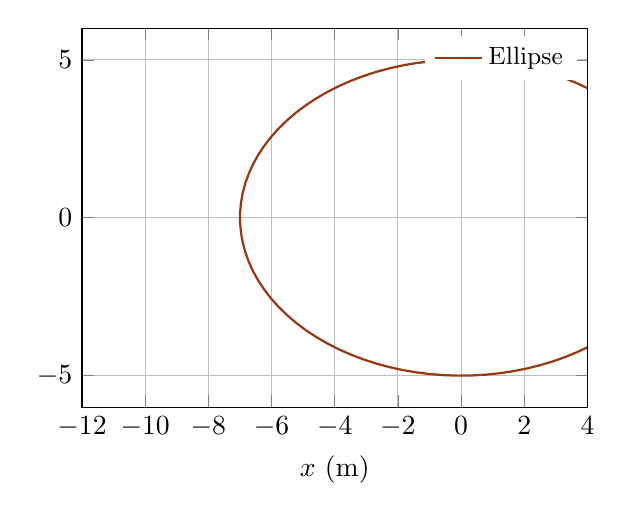
\begin{tikzpicture}
  \begin{axis}[baneplott, width=8cm, legend style={draw=none, font=\small},
               at={(0,0)}, anchor=north west]
    \addplot[rust, thick, domain=0:360, samples=100] ({7*cos(x)}, {5*sin(x)});
    \addlegendentry{Ellipse}
  \end{axis}
\end{tikzpicture}
\end{document}
